\subsection{L'authentification}
\label{subsec:auth-feature}

\paragraph{}
L'authentification mise en place doit être compatible avec le système d'authentification présent sur les services d'Altissia. C'est particulièrement facile, car c'est une authentification dite sans serveur. Cela veut dire qu'un client peut prouver son identité sans qu'un serveur tiers confirme les droits auxquels le \gls{g-client} prétend. 

\begin{figure}[h]
    \centering
    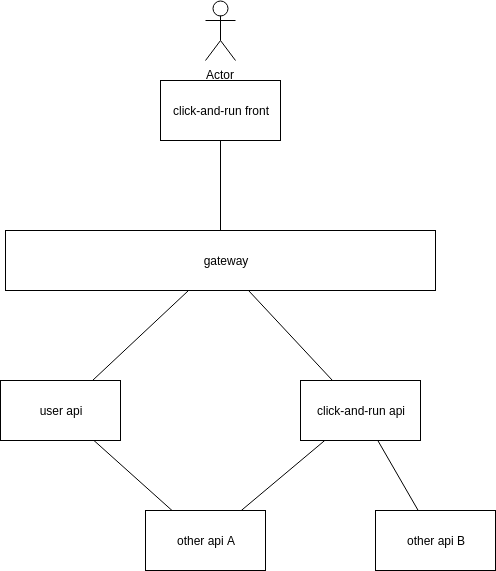
\includegraphics[width=0.7\textwidth]{images/diagrams/gw-archi.png}
    \caption{L'organisation des services et leurs communications (non \gls{a-uml})}
    \label{fig:gw-archi}
\end{figure}

\paragraph{}
Pour comprendre comment c'est possible, il faut d'abord s'intéresser à la manière dont les différents services communiquent entre eux. Comme on peut le voir sur le diagramme \ref{fig:gw-archi}, tous les \glspl{g-server} sont cachés derrière un unique point d'entrée que l'on appelle la passerelle. La passerelle vérifie que les demandes faites aux \glspl{g-server} sont authentifiées. Les demandes faites entre \glspl{g-server} ne sont pas vérifiées, car les \glspl{g-server} se font mutuellement confiance.

\begin{figure}[h]
    \centering
    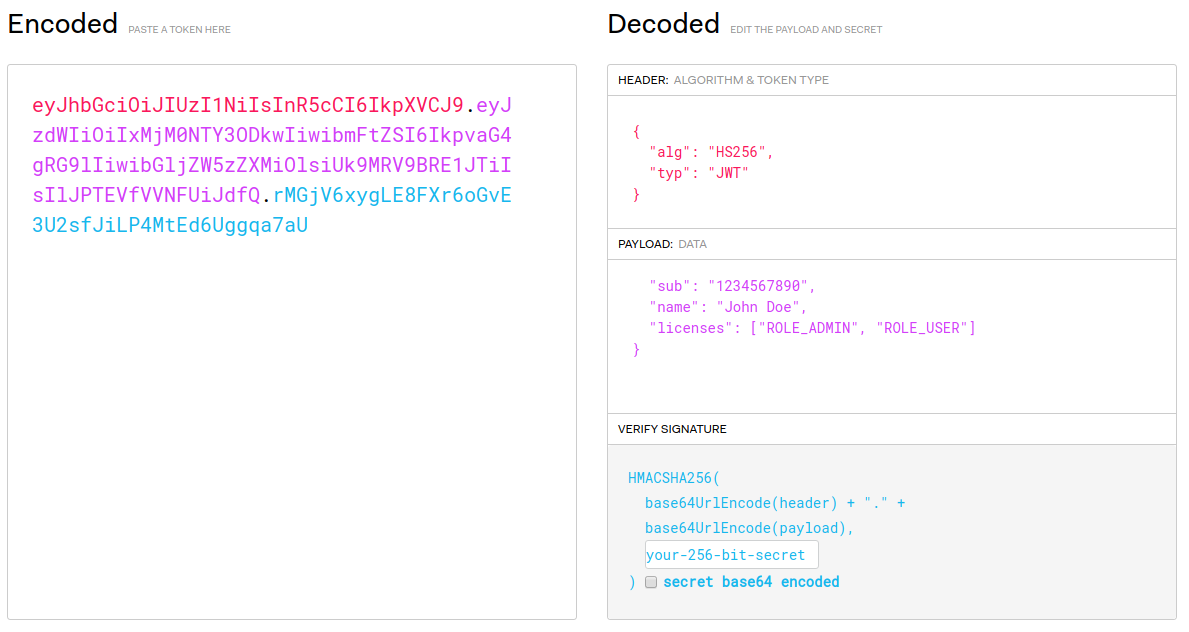
\includegraphics[width=0.7\textwidth]{images/screenshot/jwt-good-secret.png}
    \caption{Un \gls{a-jwt} à gauche et les données décodées à droite}
    \label{fig:jwt-good}
\end{figure}
\begin{figure}[h]
    \centering
    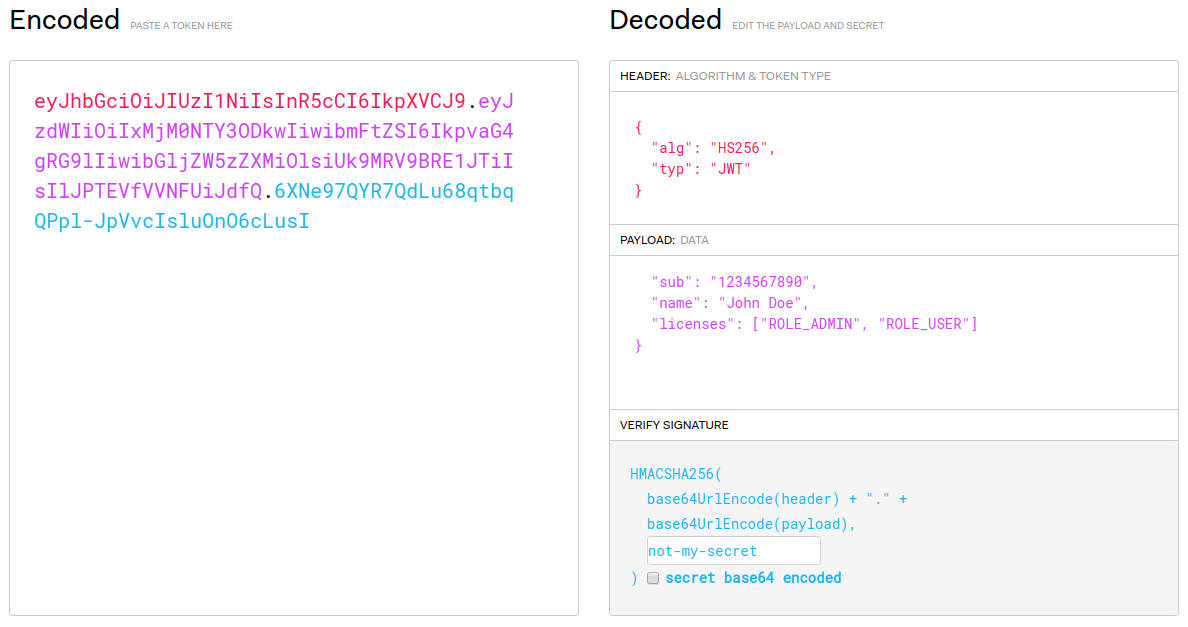
\includegraphics[width=0.7\textwidth]{images/screenshot/jwt-bad-secret.png}
    \caption{Un \gls{a-jwt} avec les mêmes données que sur la figure, \ref{fig:jwt-good} mais pas la même signature}
    \label{fig:jwt-bad}
\end{figure}

\paragraph{}
Un \gls{g-client} qui veut s'authentifier fait sa demande à la passerelle.
La passerelle consulte le service des utilisateurs et si l'identifiant et le mot de passe concordent, elle approuve l'authentification.
Elle envoie alors un \gls{a-jwt}, dont on peut observer un exemplaire sur la figure \ref{fig:jwt-good} qui est une sorte de passeport qui déclare l'identité et les droits de l'utilisateur.
Ce \gls{a-jwt} est lisible par tous et est infalsifiable. Son contenu est accompagné d'une signature qui est le résultat de ce même contenu passé par une \gls{g-hash-func}.
La seule manière de reproduire cette signature est de disposer de la \gls{g-hash-func} et du secret.
La figure \ref{fig:jwt-bad} illustre ce que l'on obtient sans le bon secret.
Cette formule est présente sur le \gls{a-jwt} et est donc accessible à tous.
Le secret lui n'est connu que par la passerelle et il n'y a donc qu'elle qui peut produire cette signature.

\paragraph{}
À chaque requête, un client accompagne sa demande de son \gls{a-jwt} et la passerelle reproduit la signature.
Si la signature produite est la même que celle inscrite sur le \gls{a-jwt}, la passerelle transmet la demande, sinon elle la rejette.
Et lorsque les \glspl{g-server} doivent communiquer entre eux pour remplir la demande du client, ils font confiance aux droits indiqués, car ils ont été vérifiés par la passerelle.

\paragraph{}
Pour que cela fonctionne, la nouvelle application cliente doit:
\begin{enumerate}
    \item Adresser toutes ses demandes à la passerelle
    \item Implémenter la demande d'authenfication
    \item Fournir le \gls{a-jwt} à chaque requête
\end{enumerate}
Tandis que le nouveau \gls{g-server} doit juste contrôler que les droits d'un utilisateur correspondent au niveau d'autorisation requise pour les ressources qu'il demande.
